% =====================================================================
%  Manuscript for IEEE Transactions on Evolutionary Computation (TEVC)
%  Build:  latexmk -pdf main.tex      (or upload this folder to Overleaf)
%  Outline: project doc 「论文提纲_v1」 (2026-10-22)
% =====================================================================
\documentclass[journal]{IEEEtran}

% ---------- packages ----------
\usepackage[T1]{fontenc}
\usepackage{cite}
\usepackage{amsmath,amssymb,amsfonts}
\usepackage{graphicx}
\usepackage{booktabs}
\usepackage{multirow}
\usepackage{array}
\usepackage{algorithm}
\usepackage{algpseudocode}
\usepackage{xcolor}
\usepackage{url}
\usepackage{xspace}
\usepackage{tikz}
\usetikzlibrary{arrows.meta,positioning,calc}
\usepackage[hidelinks]{hyperref}

\graphicspath{{figures/}}

\newtheorem{proposition}{Proposition}
\newtheorem{corollary}{Corollary}

% ---------- notation (keep all symbols here so they stay consistent) ----------
\newcommand{\K}{K}                       % deviation density / number of deviation slots
\newcommand{\dist}{d}                    % distance between rule-decoded solution and good solutions
\newcommand{\nalt}{q}                    % number of alternatives per decision
\newcommand{\HV}{\mathrm{HV}}            % hypervolume
\newcommand{\proxy}{S}                   % surrogate (proxy) score of a rule
\newcommand{\genome}{\mathbf{g}}         % genotype
\newcommand{\decoder}{\mathcal{D}}       % decoder
\newcommand{\rul}{r}                     % construction rule (\rule is a LaTeX built-in)
\newcommand{\eg}{e.g.,\ }
\newcommand{\ie}{i.e.,\ }

% ---------- drafting helpers (remove before submission) ----------
\newcommand{\todo}[1]{\textcolor{red}{[TODO: #1]}}
\newcommand{\note}[1]{\textcolor{blue}{[NOTE: #1]}}


% ---------- title ----------
% Working title (outline v1); revisit after the abstract is fixed.
\title{Rules as Bias, Deviations as Freedom:\\
Rule-Deviation Decoding for Evolutionary Rostering}

\author{%
  Author~One,~\IEEEmembership{Student Member,~IEEE,}
  and~Author~Two% TODO: real names, affiliations, funding
  \thanks{Manuscript received XXX; revised XXX.}%
  \thanks{The authors are with XXX (e-mail: XXX).}%
}

\markboth{IEEE Transactions on Evolutionary Computation,~Vol.~XX, No.~X, Month~2026}%
{Rule-Deviation Decoding for Evolutionary Rostering}

\begin{document}

\maketitle

\begin{abstract}
% 证据：第 VI 节各表。≤ 250 词（TEVC）。
Decoders for evolutionary scheduling build a solution one decision at a time and usually give every decision its own gene.
Changing one gene then changes how all later genes are read, and the decoder's bias toward good solutions cannot be tuned.
We propose rule-deviation decoding (RDD), which separates bias from freedom.
A construction rule makes every decision by default; the genotype encodes only a few deviation slots, each naming a decision and an alternative action.
The deviation rate, the expected share of decisions at which a random genotype departs from the rule, sets how far the search may move from the rule.
Rules are learned offline by scoring the solutions that random deviations produce;
genetic programming, a neural network trained by an evolution strategy, and a large language model reach similar quality under this score.
A rule-distance model shows that too few slots keep good solutions out of reach and that the best number of slots grows with the budget.
On a bi-objective robot--tool duty rostering problem, RDD raises the mean hypervolume of NSGA-II on 47 test instances from 0.570 to 0.788.
For repairs during execution, using the old roster as the rule works better than seeding the population with it.
On 276 flexible job shop benchmarks, RDD with a standard dispatching rule outperforms random keys on most instances, also with MOEA/D, larger budgets and heuristic initialization.
On both problems, the deviation rate, not the number of slots, is the parameter that matters.
\end{abstract}

\begin{IEEEkeywords}
Representation, decoder, multi-objective evolutionary algorithm, rostering, flexible job shop scheduling, heuristic bias, limited discrepancy search.
\end{IEEEkeywords}


\section{Introduction}
\label{sec:intro}

% 证据：调研笔记 01、03
% 段落计划：
%  1. 间接编码 + 解码器在调度/排班中很常见；解码器带来多对一（冗余）。
%  2. 规则（启发式）偏置有用但不稳健——好解离规则远时偏置有害（Rothlauf 的冗余/偏置理论）。
%  3. 本文问题：如何同时给出偏置与自由度，以及如何获得"好的"规则。
%  4. 本文做法概述。
%  5. 贡献列表（见下）。
%  6. 文章结构。
% 图 1：编码示意（dec5 逐班基因 vs 规则 + 稀疏偏离）

\todo{Introduction.}

The main contributions of this paper are as follows.
\begin{enumerate}
  \item \textbf{Representation.} \todo{Rules plus sparse deviation slots, with the deviation density as an explicit parameter (LDS idea turned into an MOEA encoding).}
  \item \textbf{Theory.} \todo{Bias--freedom model: for $\K<\dist$ search stalls above $\dist-\K$; small-budget optimum $\K\approx\dist$, large-budget $\approx\dist/\nalt$; multi-objective case follows the mean distance.}
  \item \textbf{Rule acquisition.} \todo{Rules should be optimized for bias quality (the proxy score); under this objective GP, neural network + ES and LLM are interchangeable; imitating good solutions is not enough.}
  \item \textbf{Applications.} \todo{Static rostering (47 test instances), mid-execution re-rostering, and public FJSP benchmarks.}
\end{enumerate}

% Organization paragraph
\todo{Organization of the paper.}

\section{Related Work}
\label{sec:related}

% 证据：调研笔记 01～03

\subsection{Redundancy and Representation Theory}
% Rothlauf 的冗余表示理论（同义冗余、偏置）；Gottlieb & Raidl 关于解码器局部性
\todo{Redundant representations and decoders \cite{rothlauf2006representations}.}

\subsection{Heuristics Combined with Genetic Perturbation}
% 问题空间/启发式空间搜索（Storer 等 1992、1995）；Hart & Ross 1998；
% LDS 1995；HBSS 1996；Aickelin & Dowsland 2004（间接 GA 护士排班）
\todo{Problem/heuristic-space search \cite{storer1992new}, LDS \cite{harvey1995lds}, HBSS \cite{bresina1996hbss}, indirect GA for nurse scheduling \cite{aickelin2004indirect}.}

\subsection{Learning Construction Rules}
% GP 超启发式综述；EoH / ReEvo / FunSearch；L2D
\todo{GP hyper-heuristics, LLM-based heuristic design \cite{romera2024funsearch}, learning to dispatch.}

\subsection{Rescheduling and Re-rostering}
% Shen & Yao 2015；护士重排班
\todo{Dynamic scheduling and re-rostering \cite{shen2015dfjsp}.}

\section{Problem Definition and Motivation}
\label{sec:problem}

% 证据：exact/mirror.py（模型、目标）；exact/family_bounds.py、robot_lb.py（下界）；tools/gen_family*.py、gen_request.py、rulegen/instances.py（实例与划分）；
%       实验0_表示分析/exp0lib.py（D0～D5）；实验0_报告.md、out/report_metrics.md、out/report_writeback.md（III-E 的数字）；排班_解码方案汇总.md（最优解结构）
% 2026-10-22 已两轮独立核对；本版只改写表达，事实未改。

This section defines the rostering problem, the instances, and the six decoders that we use as baselines.
It ends with an analysis of these decoders, which shows what a better decoder needs.

\subsection{Robot--Tool Duty Rostering}
\label{sec:problem:model}

A duty post must be staffed by one robot at all times during a horizon $[0,\horizon]$.
Robots take turns in \emph{shifts}, and each shift starts when the previous one ends.
If shift $i-1$ ends at time $E_{i-1}$ and shift $i$ is served by a robot of type $\tau$,
shift $i$ ends at $E_i = E_{i-1} + w_\tau$, where $w_\tau$ is the duty length of type $\tau$.
The first shift starts once the first robot has installed its tools and travelled to the post.
The roster is complete when $E_i \ge \horizon$.

\textbf{Robots.}
Each robot type $\tau$ has a travel time to the post $o_\tau$, a return time $b_\tau$, a charging time $\gamma_\tau$ and a maintenance time $\mu_\tau$.
A robot can serve at most $n_\tau$ duties between two maintenances; we call this its \emph{duty budget}.
After each duty the robot returns and its tools are removed.
It then charges, or, if its budget is used up, goes to maintenance, which refills the budget.
A robot is \emph{available} for a shift that starts at time $E$ if it is ready by $E - o_\tau$ and still has budget for one duty.
At most $L_\tau$ robots of type $\tau$ may be used.

\textbf{Tools.}
Each duty needs $\nu_\tau$ tools of types compatible with the robot.
A tool in use is busy for its installation, its travel and work time, its removal and a rest period.
When a robot is dispatched, the simulator first reuses compatible tools that are ready, earliest first.
If tools are missing, new ones are created, and their type has to be chosen.
At most $L_k$ tools of type $k$ may be used.
A roster is infeasible if it needs more robots or tools than these limits allow.

\textbf{Decisions.}
At every shift $i$ one decision is made: which robot serves it.
The decision is an action
\begin{equation}
  \act_i \in \{\reuse(r) : r \in \avail_i\} \cup \{\new(\tau)\},
\end{equation}
where $\avail_i$ is the set of available robots.
\reuse{}$(r)$ sends a robot that is already in the fleet; \new{}$(\tau)$ adds a new robot of type $\tau$.
Together with the types of the new tools, these actions fix the roster.
Each action changes which robots are available later, so a decision at one shift affects all later shifts.

\subsection{Objectives}
\label{sec:problem:objectives}

We minimize two objectives.
The first is the \emph{resource count}, the number of robots and tools used:
\begin{equation}
  \fres = |\mathcal{R}| + |\mathcal{T}|.
\end{equation}
The second is the \emph{imbalance} of the robot fleet:
\begin{equation}
  \fbal = 0.3\,\sigma(\mathbf{n}) + 0.4\,\sigma(\mathbf{h}) + 0.3\,\sigma(\Delta\mathbf{t}),
\end{equation}
where $\sigma(\cdot)$ is the standard deviation, $\mathbf{n}$ and $\mathbf{h}$ are the robots' duty counts and total duty hours,
and $\Delta\mathbf{t}$ are the gaps between the times at which successive robots first go to maintenance.
A low imbalance means that all robots wear evenly and do not go to maintenance at the same time.
The two objectives conflict.
A small fleet must work some robots hard, while an even workload needs extra robots.

For each instance we also compute a lower bound $\LB$ on the resource count.
The robot part comes from an exact feasibility search with unlimited tools;
the tool part checks whether a tool used in one shift can be ready again for the next shift, and if not, counts the extra tools needed.

\subsection{Instances}
\label{sec:problem:instances}

We use 62 instances (Table~\ref{tab:instances}).
Four are hand-built scenarios: one is the request file of the scheduling software that motivated this work (one robot type, 700\,h),
and three have three robot types and four tool types, one of them with tight fleet limits.
The other 58 are random instances in three families:
\begin{itemize}
  \item \textbf{E} (homogeneous): one robot type.
  \item \textbf{H} (heterogeneous): two or three robot types, all with 10\,h duties.
  \item \textbf{M} (mixed duty lengths): two or three robot types with duty lengths from $\{6,8,10,12\}$\,h, so shifts have different lengths.
\end{itemize}
Robot parameters are drawn at random: travel 1--2\,h, charging 2--5\,h, maintenance 48--120\,h,
2--5 duties per maintenance cycle, 2 or 3 tools per duty, and 6--10 robots per type.
Tools take 1--2\,h to install or remove and rest for 3--8\,h.
We generated 60 random instances and removed two for which no method found a feasible roster.

The instances are split once into 15 training instances (five per family) and 47 test instances.
The construction rules of our method are learned on the training instances only, and its deviation density is selected on them (Section~\ref{sec:method}).
The test instances measure the final performance.
% 待定（κ 完整结果出来后再写）：是否说明早期探索性运行曾在测试集上评价过 κ = 0.5

\begin{table}[t]
  \centering
  \caption{Instance groups. $\Nmax$ is the upper bound on the number of shifts.}
  \label{tab:instances}
  \footnotesize
  \setlength{\tabcolsep}{2.5pt}
  \begin{tabular}{@{}lccccccc@{}}
    \toprule
    Group & Train & Test & \shortstack{Robot\\types} & \shortstack{Tool\\types} & Horizon (h) & Duty (h) & $\Nmax$ \\
    \midrule
    Hand-built & 0 & 4  & 1--3 & 1--4 & 700--1440 & 6, 10 & 70--240 \\
    E        & 5 & 12 & 1    & 1--3 & 480--1080 & 10    & 48--108 \\
    H        & 5 & 15 & 2--3 & 2--3 & 480--1080 & 10    & 48--108 \\
    M        & 5 & 16 & 2--3 & 2--3 & 480--1080 & 6--12 & 60--180 \\
    \midrule
    Total    & 15 & 47 & & & & & \\
    \bottomrule
  \end{tabular}
\end{table}

\subsection{Encoding and Baseline Decoders}
\label{sec:problem:decoders}

All decoders in this paper use a random-key genotype $\genome \in [0,1)^n$, a vector of $n$ numbers, and build the roster one shift at a time.
At each shift the decoder finds the available robots, picks an action, and simulates the shift.
Since every shift lasts at least $\min_\tau w_\tau$, the number of shifts is at most
\begin{equation}
  \Nmax = \left\lceil \horizon / \min_\tau w_\tau \right\rceil .
\end{equation}

The baseline decoders give each shift two genes: a robot gene $x_i$ that picks the action, and a tool gene $y_i$ that picks the type of any new tool.
The tool gene points into the list of the $c_\tau$ compatible types at position $\lfloor y_i (c_\tau - 1) \rfloor$;
if that type has reached its limit, the next type is used.
All decoders read the tool genes in this way, following the original software.
They differ in how they read the robot gene.
We name them \dec{0} to \dec{5}; each one adds a piece of problem knowledge to the one before.

\textbf{\dec{0} (original).}
The gene is scaled to an index over the available robots followed by the robot types: $\lfloor (x_i - 10^{-3})(|\avail_i| + n_R) \rfloor$, where $n_R$ is the number of types.
A small index sends an available robot, and a large one opens a new robot.
Because $|\avail_i|$ changes from shift to shift, the same gene value can mean ``send'' at one shift and ``open'' at another.

\textbf{\dec{1} (threshold).}
A gene below $\theta = 0.85$ always means \reuse, and a gene above $\theta$ always means \new.
Below $\theta$, the gene picks robot $\lfloor x_i |\avail_i| / \theta \rfloor$; above $\theta$, it picks a type.

\textbf{\dec{2} (ranking).}
As \dec{1}, but the available robots are sorted, fewest duties first (ties: most remaining budget first).
A small gene now sends the least-used robot.

\textbf{\dec{3} (capacity look-ahead).}
As \dec{2}, but before opening a new robot the decoder estimates how many duty hours the current fleet can still provide.
If the fleet can cover the rest of the horizon, it sends an existing robot instead.

\textbf{\dec{4} (maintenance phase).}
As \dec{3}, but robots that are closest to maintenance are ranked first.

\textbf{\dec{5} (backtracking repair).}
As \dec{3}, with one more step.
If no robot is available at shift $i$, the decoder goes back over the last $W = 12$ shifts.
At each of them it tries sending a different robot and re-simulates up to shift $i$.
It keeps the first change that leaves a robot available at shift $i$, and opens a new robot only if no change works.

\dec{5} performs best of the six and is our main baseline.
All six decoders, however, share one structure: every shift has its own gene, and that gene decides the shift.
We implemented all decoders in Python and checked \dec{1}--\dec{5} against the C++ code of the original software, genotype by genotype.

\subsection{Motivation: What the Baseline Decoders Show}
\label{sec:motivation}

To see why some decoders work better than others, we measured four properties of each decoder on 16 instances
(the four hand-built scenarios with all six decoders, and 12 E, H and M instances with \dec{2}--\dec{5}):
\begin{itemize}
  \item \textbf{Neutral rate}: the chance that redrawing one robot gene leaves the roster unchanged.
  A high neutral rate means that many genotypes produce the same roster, \ie the encoding is \emph{redundant}.
  \item \textbf{Good-start rate}: the chance that a uniformly random genotype gives a roster with $\fres \le \LB + 1$.
  \item \textbf{Change propagation}: after one robot gene is changed, the share of later shifts whose robot also changes.
  \item \textbf{Reachability}: whether some genotype produces the optimal roster. We computed the optimal rosters of the hand-built scenarios by dynamic programming.
\end{itemize}
We also recorded the \emph{override share}: how often the capacity look-ahead of \dec{3}--\dec{5} (below) turns a \new action into a \reuse action.
The good-start rate is estimated from 1000 random genotypes.
The neutral rate and change propagation are measured on 100 random feasible genotypes and on the 30 best of the 1000, with five single-gene changes each.
We then compared these properties with the hypervolume (HV) that NSGA-II \cite{deb2002nsga2} reaches with each decoder
(population 30, about 465 evaluations).
For each instance we computed the Spearman correlation between each property and HV across the decoders, and we report the median over instances.
Table~\ref{tab:neutral} lists the first two properties on the hand-built scenarios.

\begin{table}[t]
  \centering
  \caption{Neutral rate / good-start rate of the six decoders on the four hand-built scenarios.}
  \label{tab:neutral}
  \footnotesize
  \setlength{\tabcolsep}{1.6pt}
  \begin{tabular}{@{}lcccccc@{}}
    \toprule
    Scenario & \dec{0} & \dec{1} & \dec{2} & \dec{3} & \dec{4} & \dec{5} \\
    \midrule
    1 type, 700 h   & 0.30/.000 & 0.42/.007 & 0.41/.007 & 0.61/.919 & 0.61/.929 & 0.69/.981 \\
    3 types, 720 h  & 0.10/.000 & 0.21/.000 & 0.22/.000 & 0.44/.020 & 0.46/.024 & 0.50/.032 \\
    3 types, 1440 h & 0.06/.000 & 0.13/.000 & 0.14/.000 & 0.38/.014 & 0.42/.008 & 0.44/.029 \\
    3 types, tight  & 0.12/.000 & 0.24/.000 & 0.19/.000 & 0.44/.020 & 0.47/.024 & 0.49/.032 \\
    \bottomrule
  \end{tabular}
\end{table}

\textbf{Finding 1: the better decoders favor good rosters.}
From \dec{0} to \dec{5}, the neutral rate rises from 0.06--0.30 to 0.44--0.69, and the good-start rate rises with it.
Both go with better HV: the median correlation is $+0.91$ for the neutral rate and $+0.80$ for the good-start rate,
with the same sign on every instance where the correlation is defined (12/12 and 14/14).
The override share correlates even more strongly ($+0.97$, 16/16).
These three properties rise together, so the data cannot tell their effects apart.
Taken together, they agree with the theory of redundant representations \cite{rothlauf2006representations}:
an encoding helps when its redundancy favors good solutions.

\textbf{Finding 2: change propagation is high in every decoder.}
On the hand-built scenarios, changing one gene changes the robot at 39--61\% of the later shifts, for every decoder.
This share does not track performance (median correlation $+0.23$, same sign on 7/12 instances).
The reason is structural: a changed decision changes which robots are available, and every later gene is then read in a different situation.
None of the steps from \dec{0} to \dec{5} reduced this effect.

\textbf{Finding 3: built-in knowledge helps even when it hides good rosters.}
The capacity look-ahead of \dec{3}--\dec{5} sometimes forbids opening a robot.
On two hand-built scenarios, this makes the optimal roster unreachable: that roster opens a fifth robot at shift 9, which the look-ahead does not allow.
Other optimal rosters can still be reached, and on one of the two scenarios \dec{5} still finds the optimal values.
Making the optimal roster reachable again did not help.
When we added a range of gene values that always opens a robot, the imbalance got significantly worse on the two scenarios that had not lost the optimum,
and nothing improved on the two that had.

\textbf{Finding 4: well-balanced rosters are rare.}
With every decoder, at most 1.7\% of random genotypes give a roster with $\fres = \LB$ and an imbalance within 1.5 times the optimum;
on the three-type scenarios almost none do.
This is where the search falls short: at $\fres = \LB$, the mean imbalance reached by \dec{5} is 1.1--2.3 times the optimum.

\textbf{Structure of optimal rosters.}
The optimal rosters follow a simple pattern.
In 85--90\% of their shifts they send the available robot with the fewest duties.
In the remaining shifts they send a different robot; in the single-type scenario, this happens in 10 of its 65 reuse decisions.
A per-shift encoding has no direct way to say ``follow this rule except at a few shifts''.
The choice of rule also matters.
On the four hand-built scenarios, always sending the robot with the fewest duties needs 11--17 resources,
while always sending the robot with the least remaining budget reaches the lower bound of 9 on all four.

\textbf{What a better decoder needs.}
These results lead to three requirements:
\begin{enumerate}
  \item The encoding should express ``a rule plus a few exceptions'' directly: the genes should say only where and how to depart from the rule.
  \item How strongly the decoder favors the rule should be adjustable, because the distance between the rule and good rosters differs between rules and instances.
  \item The rule should be chosen for the rosters that the search finds around it, not only for the single roster it builds.
\end{enumerate}
Section~\ref{sec:method} presents a decoder that meets these requirements.

\section{Rule-Deviation Decoding}
\label{sec:method}

% 证据：rulegen/ruledec.py、neural/ruledec_ext.py（排班解码）；bench/fjsp2.py、fjsp_base3.py（FJSP：sp 均匀备选、spr 规则组合备选）；
%       evalrule.py（代理分）；neural/gp.py、nnrule.py、es.py、train_il.py；rulegen.py（LLM）；实验5续文档（ρ 的选取）。
% 2026-10-27 按新框架重写：加入备选动作集 A(s)、与优化器无关；学习器细节移到补充材料 S-IV。

\subsection{Overview}
\label{sec:method:overview}

\RDD divides the work between a construction rule and the genotype.
The rule makes every decision by default.
The genotype does not encode every decision.
It encodes a few \emph{deviations}: the decisions at which the decoder should not follow the rule, and what it should do there instead.
Fig.~\ref{fig:framework} shows how \RDD is used.
A rule is learned offline on training instances (Section~\ref{sec:method:learn}).
An MOEA then searches over the deviations, and every genotype it creates is decoded relative to the rule.

\begin{figure*}[t]
  \centering
  \figplaceholder{5.2cm}{Fig.~2 (framework, to be drawn): (1) offline rule learning with the proxy score; (2) online search with the RDD decoder and the deviation rate $\rho$; (3) applications: static rostering, re-rostering, flexible job shop.}
  \caption{Overview of rule-deviation decoding. A rule is learned offline by scoring the solutions that random deviations from it produce. An MOEA then searches over deviation slots; the decoder follows the rule wherever no slot is active.}
  \label{fig:framework}
\end{figure*}

\subsection{Rules and Alternatives}
\label{sec:method:rule}

A schedule is built one decision at a time.
At decision $i$ the decoder is in state $s_i$, and the rule $\rul$ returns its first choice $\rul(s_i)$.
A deviation replaces this choice by an action from an \emph{alternative list} $A(s_i)$.
The alternative list is part of the design.
We use two kinds:
\begin{itemize}
  \item \textbf{Ranked alternatives.} $A(s_i)$ holds all other feasible actions in the rule's order.
  This suits problems with few feasible actions per decision.
  We use it in rostering, where a deviation either sends one of the few other available robots or opens a new robot.
  \item \textbf{Rule portfolio.} A few other rules each propose their first choice, and $A(s_i)$ holds these proposals.
  A proposal may coincide with the rule's choice; the deviation then has no effect.
  This suits problems with many feasible actions, most of them poor.
  We use it in the flexible job shop, where a decision chooses among dozens of operation--machine pairs and many standard dispatching rules exist.
\end{itemize}
In both cases a deviation picks one entry of the list, and under random genes every entry is equally likely.
What matters is that the entries are reasonable candidates.
On the flexible job shop, a rule portfolio is clearly better than ranked alternatives over all operation--machine pairs (Section~\ref{sec:exp-ablation}).

In rostering, the rule sees the current time, the available robots, and for every robot its duty count, hours, remaining budget, duties left before maintenance and ready time.
It also sees the parameters of each robot type and a \emph{gene type} $\tau_g$, a robot type read from one gene, which the rule may use when it opens a robot.
The simplest rule is the \emph{default rule} $\rul_0$: send the available robot with the fewest duties, and open a robot of type $\tau_g$ if none is available.

\subsection{Genotype and Decoding}
\label{sec:method:genotype}

The genotype holds $\K$ \emph{deviation slots}, two genes per slot, in $[0,1)$:
\begin{equation}
  \genome = (p_1, a_1, \dots, p_\K, a_\K, \text{other genes}).
\end{equation}
In rostering, the other genes are the gene type $g$ and one tool gene per shift, read as in the baselines; FJSP needs no other genes.
The number of slots grows with the number $N$ of decisions, $\K = \max(4, \lceil \dens N \rceil)$, where $\dens$ is the \emph{slot ratio}.
Each slot works as follows:
\begin{itemize}
  \item \textbf{On or off.} The slot is active if $a_k \ge 1 - \qon$, where $\qon$ is the \emph{activation probability}.
  \item \textbf{Where.} An active slot acts on decision $\lfloor p_k N \rfloor$. If two active slots hit the same decision, the later one counts.
  \item \textbf{What.} The value $u_k = (a_k - 1 + \qon)/\qon \in [0,1)$ picks an alternative from $A(s)$ by its position in the set.
\end{itemize}
Algorithm~\ref{alg:decode} lists the decoder.
It collects the active slots, then builds the schedule decision by decision.
At a decision with an active slot it takes the chosen alternative, if that action is feasible; otherwise it takes the rule's first choice.
In rostering the alternatives are split as in the baselines: values $u_k < 0.85$ send another robot and larger values open a new robot of a type chosen by $u_k$;
the decoder also keeps the capacity check and the backtracking repair of \dec{5} on decisions without a deviation.

\begin{algorithm}[t]
  \caption{Rule-deviation decoding}
  \label{alg:decode}
  \begin{algorithmic}[1]
    \Require genotype $\genome$, rule $\rul$, alternative lists $A(\cdot)$, slot ratio $\dens$, activation probability $\qon$
    \Ensure a schedule, or \textsc{infeasible}
    \State $\K \gets \max(4, \lceil \dens N \rceil)$;\ \ $\Delta \gets \emptyset$
    \For{$k = 1, \dots, \K$}
      \If{$a_k \ge 1 - \qon$} \State $\Delta[\lfloor p_k N \rfloor] \gets (a_k - 1 + \qon)/\qon$ \EndIf
    \EndFor
    \State $s \gets$ initial state
    \For{$i = 0, 1, \dots$ until the schedule is complete}
      \State $\act \gets \rul(s)$
      \If{$i \in \Delta$}
        \State $\act' \gets$ element of $A(s)$ at position $\lfloor \Delta[i]\, |A(s)| \rfloor$
        \If{$\act'$ is feasible in $s$} $\act \gets \act'$ \EndIf
      \EndIf
      \State $s \gets$ apply $\act$ to $s$
      \If{a resource limit is exceeded} \Return \textsc{infeasible} \EndIf
    \EndFor
    \State \Return the schedule in $s$
  \end{algorithmic}
\end{algorithm}

The key difference from per-decision encodings lies in what happens after a change.
In a per-decision encoding, a changed decision changes the state, and every later gene is then read in this new state, often with a new meaning.
In \RDD, most later decisions have no gene.
The rule makes them, and it adapts to the new state.
Fig.~\ref{fig:encoding} illustrates this on ten shifts.

\begin{figure}[t]
  \centering
  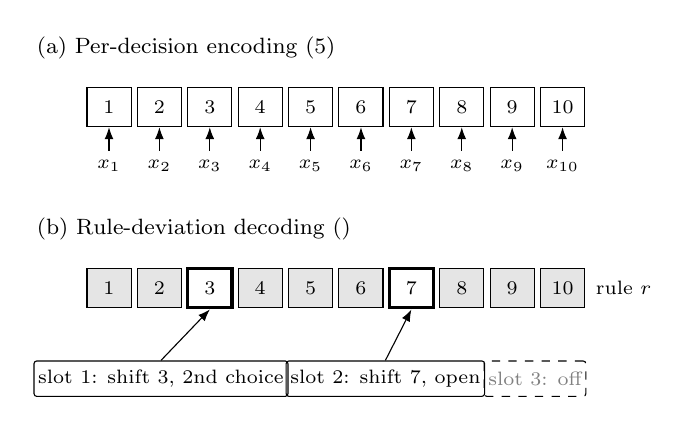
\begin{tikzpicture}[
      sh/.style={draw, minimum width=5.6mm, minimum height=5mm, inner sep=0pt, font=\scriptsize},
      gn/.style={font=\scriptsize},
      sl/.style={draw, rounded corners=1pt, minimum height=4.5mm, inner sep=1.5pt, font=\scriptsize},
      ar/.style={-{Latex[length=1.5mm]}, thin}]
    \node[font=\footnotesize, anchor=west] at (-0.4,0.75) {(a) Per-decision encoding (\dec{5})};
    \foreach \i in {1,...,10} {
      \node[sh] (a\i) at (0.64*\i,0) {\i};
      \node[gn] (x\i) at (0.64*\i,-0.75) {$x_{\i}$};
      \draw[ar] (x\i) -- (a\i);
    }
    \node[font=\footnotesize, anchor=west] at (-0.4,-1.55) {(b) Rule-deviation decoding (\RDD)};
    \foreach \i in {1,2,4,5,6,8,9,10} {
      \node[sh, fill=black!10] (b\i) at (0.64*\i,-2.3) {\i};
    }
    \node[sh, very thick] (b3) at (0.64*3,-2.3) {3};
    \node[sh, very thick] (b7) at (0.64*7,-2.3) {7};
    \node[sl] (s1) at (1.3,-3.45) {slot 1: shift 3, 2nd choice};
    \node[sl] (s2) at (4.15,-3.45) {slot 2: shift 7, open};
    \node[sl, dashed, text=black!50] (s3) at (6.05,-3.45) {slot 3: off};
    \draw[ar] (s1.north) -- (b3.south);
    \draw[ar] (s2.north) -- (b7.south);
    \node[font=\scriptsize, anchor=west] at (6.7,-2.3) {rule $\rul$};
  \end{tikzpicture}
  \caption{Two encodings of a ten-shift roster. (a) Each shift has its own gene. (b) Gray shifts follow the rule $\rul$; the genotype holds deviation slots, here two active ones that change shifts 3 and 7.}
  \label{fig:encoding}
\end{figure}

\subsection{The Deviation Rate}
\label{sec:method:rate}

In a uniformly random genotype, each slot is active with probability $\qon$, so about $\qon\K \approx \qon\dens N$ slots are active.
We call
\begin{equation}
  \drate = \qon\dens
\end{equation}
the \emph{deviation rate}, the expected number of active slots per decision.
It sets the balance between bias and freedom.
A small $\drate$ keeps random genotypes close to the rule's schedule; a large $\drate$ lets them spread far from it.
On both problems, settings with the same $\drate$ but different $\dens$ and $\qon$ perform alike (Section~\ref{sec:experiments}), so $\drate$ is the parameter to set.
The realized share of decisions that differ from the rule is smaller than $\drate$, because several slots may hit the same decision and an alternative may coincide with the rule's choice.

Two existing encodings are limiting cases of \RDD.
A per-decision encoding that ranks the options by a rule corresponds to one gene for every decision and no default: every decision is free.
Heuristic-space search \cite{storer1992new,dorndorf1995evolution}, which picks a rule for every decision, corresponds to a rule portfolio with no default rule.
\RDD adds what both lack: a default, and a parameter that sets how often the search may leave it.

\textbf{Optimizer.}
\RDD is an encoding, so any optimizer for real-valued genotypes can use it.
Our main experiments use NSGA-II \cite{deb2002nsga2}.
We also report MOEA/D \cite{zhang2007moead} and a Pareto local search that, starting from the rule's schedule, repeatedly redraws $j$ random slots of an archived solution.

\subsection{Learning the Rule}
\label{sec:method:learn}

In \RDD the rule is used inside a search.
A good rule is therefore not simply one that builds a good schedule on its own.
It is one near which the search finds good schedules.
We measure this with a \emph{proxy score}.
For each training instance $I$ we fix a set $G_I$ of 67 genotypes: three with all slots off and 64 uniformly random ones.
Let $\mathcal{D}_\rul(\genome)$ be the solution that \RDD decodes from $\genome$ with rule $\rul$. The proxy score is
\begin{equation}
  \proxy(\rul) = \frac{1}{|\mathcal{I}_{\text{train}}|} \sum_{I \in \mathcal{I}_{\text{train}}} \HV_I\bigl(\{\mathcal{D}_\rul(\genome) : \genome \in G_I\}\bigr),
\end{equation}
where $\HV_I$ is the hypervolume of the non-dominated feasible solutions, with the objectives normalized per instance by the solutions of the default rule $\rul_0$.
All rules are scored on the same genotypes, so differences between rules are not due to sampling.
One evaluation of $\proxy$ costs $15 \times 67 = 1005$ decodings.
During learning we use $\drate = 0.1$.

The proxy score treats the rule as a black box, so any kind of rule can be optimized with it.
We use three learners; their settings are given in Section~S-IV of the supplementary material.
\begin{itemize}
  \item \textbf{GP.} Two trees score \reuse and \new candidates from 22 and 17 size-independent features of the state and the candidate (population 64, 30 generations).
  \item \textbf{Neural network + ES (ES16).} A network with 16 hidden units scores each candidate from 27 features.
  It is first trained to imitate good rosters found by \dec{5}, which gives a useful starting point, and then OpenAI-ES \cite{salimans2017evolution} optimizes $\proxy$ directly.
  \item \textbf{LLM.} An LLM writes the rule as a Python function. We evolve it in the style of EoH \cite{liu2024evolution} for 12 generations, showing the LLM the score of each rule; one run needs about 55 LLM calls.
\end{itemize}
For FJSP we do not learn a rule; we use a standard dispatching rule.

\subsection{Setting the Deviation Rate}
\label{sec:method:k}

The best deviation rate depends on how far good solutions lie from the rule and on the budget (Section~\ref{sec:theory}).
Neither is known for a new instance, so we set $\drate$ once on training instances, with a selection procedure fixed before the runs.
For rostering, each candidate setting was run with the eight GP and ES16 rules on the 15 training instances,
and the setting with the highest mean HV was kept.
We first compared $\drate = 0.1$ to $0.4$ with $\qon = 0.4$, and then $\qon = 0.4$, 0.6 and 0.8 at the largest slot ratio.
The procedure selected $\drate = 0.4$ ($\dens = 1.0$, $\qon = 0.4$).\footnote{Before this selection, an exploratory run had evaluated $\drate = 0.2$ on the test instances. The final rate was chosen on the training instances only; test results at other rates are reported only as a sensitivity analysis.}
For FJSP, the settings of \RDD and of all compared methods were chosen in the same way on 15 instances that are not used in the comparison (Section~\ref{sec:exp-fjsp}).

\section{Theoretical Analysis}
\label{sec:theory}

% 证据：实验 6a（theory/model.py、sweep.py、sweep.json、meanfield.py）；T11 报告（bias_multi.py，检验 B、D；t11_tables.md）
% 不能写："理论预言了 K0.5"；区间比例 1/q 在 FJSP 上未定量验证（只在实验节写定性结论）
% 2026-10-22 命题 1～3、推论、K* = 12/26/55、表格数字均已独立核对；本版只改写表达，事实未改。
% 待补（T12 结果出来后再写）：冗余解码是否降低多余偏离的代价

How many deviation slots should \RDD use?
Too few, and the search cannot reach rosters that differ from the rule in many shifts.
Too many, and random genotypes contain many unnecessary deviations, so the search starts far from the rule and wastes evaluations removing them.
This section makes the trade-off precise with a simple model.
The model shows that the best number of slots depends on two quantities:
how many decisions separate a good solution from the rule, and how many evaluations the search can spend.

\subsection{Model}
\label{sec:theory:model}

A solution is a string $\mathbf{z} \in \{0, \dots, \nval-1\}^{\npos}$ of $\npos$ decisions with $\nval$ options each.
Option 0 is the rule's choice, so the rule's solution is the all-zero string.
A target solution $\mathbf{z}^\ast$ differs from the rule in $\dist$ positions.
We call $\dist$ the \emph{rule distance}.
The objective is the number of positions in which a solution differs from the target, $f(\mathbf{z}) = |\{j : z_j \ne z^\ast_j\}|$.
In this model, changing one decision does not change the meaning of other decisions.
Section~\ref{sec:motivation} found that this kind of propagation did not explain performance differences between decoders.

We compare two encodings with genes in $[0,1)$:
\begin{itemize}
  \item \textbf{Per-shift (PS)}: one gene per decision, read as $z_j = \lfloor g_j \nval \rfloor$.
  This is a simplified, unbiased version of \dec{0}--\dec{5}; the real decoders lean toward the rule's choice more than PS does.
  \item \textbf{Sparse deviation (SP$_\K$)}: the model version of \RDD, with $\K$ slots as in Section~\ref{sec:method:genotype}.
  A slot is on with probability $\qon \approx 0.4$ in a random genotype.
  An active slot sets one position, chosen by $p_k$, to a non-zero option chosen by $a_k$.
  If two slots hit the same position, the later one counts.
\end{itemize}

\subsection{Where the Search Starts and What It Can Reach}
\label{sec:theory:props}

We first look at three properties of the encoding itself, before any search.
The first is how far a random genotype is from the target.

\begin{proposition}[Starting distance]
\label{prop:init}
For a uniformly random genotype, let $\pi = 1 - (1 - \qon/\npos)^\K$ be the probability that a given position is changed by some slot. Then
\begin{equation}
  \mathbb{E}[f_{\mathrm{SP}}] = (\npos - \dist)\,\pi + \dist \left(1 - \frac{\pi}{\nval-1}\right).
\end{equation}
For PS, $\mathbb{E}[f_{\mathrm{PS}}] = \npos (1 - 1/\nval)$.
\end{proposition}

\begin{IEEEproof}
Each slot hits a given position with probability $\qon/\npos$, independently of the other slots, so the position is changed with probability $\pi$.
The last write at a changed position is uniform over the $\nval-1$ non-zero options.
A position where the target agrees with the rule is wrong exactly when it is changed.
A position where the target differs from the rule is right exactly when it is changed to the right option, which has probability $\pi/(\nval-1)$.
\end{IEEEproof}

When $\K$ and $\dist$ are small compared with $\npos$, this is about $\dist + \qon\K$, which depends on $\K$ and $\qon$ only through $\qon\K$, the expected number of active slots:
a random genotype is about as far from the target as the rule is, plus roughly one wrong change per active slot.
Under PS, a random genotype is $\npos(1-1/\nval)$ away, whatever the rule is; for $\npos = 100$ and $\nval = 4$ this is 75.

The second property is a hard limit.

\begin{proposition}[Reach]
\label{prop:floor}
A genotype of SP$_\K$ changes at most $\K$ positions, so no genotype gets closer to the target than $\max(0, \dist - \K)$.
\end{proposition}

With fewer slots than the rule distance, the target cannot be reached, however long the search runs.

The third property counts how many genotypes produce the target.
The more genotypes that do, the easier the target is to find.

\begin{proposition}[How often the target is represented]
\label{prop:red}
The probability that a uniformly random genotype of SP$_\K$ produces exactly $\mathbf{z}^\ast$ is
\begin{equation}
  r(\K) = \frac{\dist!}{(\nval-1)^{\dist}} \sum_{J=\dist}^{\K} \binom{\K}{J} \qon^J (1-\qon)^{\K-J} \npos^{-J}\, \mathcal{S}(J, \dist),
\end{equation}
where $\mathcal{S}(J,\dist)$ is the Stirling number of the second kind. In particular, $r(\K) = 0$ for $\K < \dist$.
\end{proposition}

\begin{IEEEproof}
Let $J$ be the number of active slots; $J$ is binomial with parameters $\K$ and $\qon$.
The genotype produces $\mathbf{z}^\ast$ exactly when all $J$ active slots fall on the $\dist$ target positions,
every target position is hit, and the last write at each one is the right option.
Of the $\npos^J$ equally likely placements, $\dist!\,\mathcal{S}(J,\dist)$ cover all $\dist$ positions.
Each of the $\dist$ last writes is right with probability $1/(\nval-1)$.
\end{IEEEproof}

\begin{corollary}
\label{cor:kstar}
Keeping only the leading term $J = \dist$, $r(\K+1)/r(\K) = (\K+1)(1-\qon)/(\K+1-\dist)$, which is at least one exactly when $\K + 1 \le \dist/\qon$.
The target is therefore represented most often when $\K$ is close to $\K^\ast \approx \dist/\qon$.
\end{corollary}

The exact maximizers agree.
For $\npos = 100$, $\nval = 4$ and $\qon = 0.4$, they are $\K^\ast = 12$, 26 and 55 for $\dist = 5$, 10 and 20, against $\dist/\qon = 12.5$, 25 and 50.
Under PS, the target is produced with probability $\nval^{-\npos}$, independent of the rule.

In short: with $\K < \dist$ the target is out of reach;
near $\K = \dist/\qon$ it is produced most often;
with more slots, random genotypes make too many wrong changes, and both the starting distance and the chance of producing the target get worse.

\subsection{The Best Number of Slots for a Given Budget}
\label{sec:theory:budget}

The three properties describe the encoding, not the search.
To find the best $\K$ for a given number of evaluations, we run a GA with the same operators as our NSGA-II (Section~\ref{sec:exp-setup}):
simulated binary crossover (SBX, $\eta = 20$, probability 0.9), polynomial mutation ($\eta = 20$, rate $1/n$ for a genotype of length $n$), population 30 and truncation selection.
We use $\npos = 100$ and $\nval = 4$, nine rule distances between 0 and 80, eleven values of $\K$ between 5 and 100, and 20 runs per setting.

Table~\ref{tab:theory-budget} shows that the best $\K$ grows with the budget:
\begin{itemize}
  \item With 465 evaluations and $\dist \le 40$, the best $\K$ is at most $\dist$.
  \item With 2000 evaluations, it is larger than $\dist$, and close to $\dist/\qon$ when $\dist$ is small.
  \item With 10\,000 evaluations, it is larger than $\dist/\qon$: 20, 50 and 75 for $\dist = 5$, 10 and 20.
\end{itemize}
No single value of $\K$ is good for all budgets.
For example, $\K = 25$ is the best choice in only one of the twelve settings of the table;
with $\dist = 40$ and 10\,000 evaluations it ends 29.7 positions from the target, while $\K = 100$ ends 12.1 away.
PS is far behind whenever $\dist \le 60$: it is still more than 40 positions away after 10\,000 evaluations.

\begin{table}[t]
  \centering
  \caption{Best number of slots $\K$ in the model ($\npos = 100$, $\nval = 4$, $\qon \approx 0.4$). Entries: best $\K$ (final distance to the target), mean of 20 runs.}
  \label{tab:theory-budget}
  \setlength{\tabcolsep}{4pt}
  \begin{tabular}{@{}rrccc@{}}
    \toprule
    $\dist$ & $\dist/\qon$ & 465 evals & 2000 evals & 10\,000 evals \\
    \midrule
    5  & 12.5 & 5 (4.0)       & 15 (3.5)  & 20 (2.4) \\
    10 & 25   & 5, 10 (8.6)   & 25 (6.8)  & 50 (3.8) \\
    20 & 50   & 10 (17.2)     & 30 (13.6) & 75 (6.8) \\
    40 & 100  & 20, 30 (35.1) & 60 (27.1) & 100$^\dagger$ (12.1) \\
    \bottomrule
    \multicolumn{5}{@{}l}{\footnotesize $^\dagger$Largest value tested.}
  \end{tabular}
\end{table}

\subsection{Why More Evaluations Call for More Slots}
\label{sec:theory:meanfield}

A simple model of the search dynamics explains this trend.
At any time, each slot is in one of three states:
on and wrong (it changes a position that should not change, or sets a wrong option), on and right, or off.
Let $w$, $c$ and $v = \K - w - c$ be the numbers of slots in these states, so that $f = w + (\dist - c)$.
Mutation changes about one gene per offspring, so each slot is touched with probability about $1/\K$.
Selection keeps only changes that lower $f$.
There are three such changes: switching off a wrong slot ($w \to w-1$),
switching on an inactive slot at a missing position with the right option ($c \to c+1$),
and moving a wrong slot to a missing position with the right option ($w \to w-1$, $c \to c+1$).
They occur at the rates
\begin{equation}
  \alpha\, \frac{w}{2\K}, \qquad
  \alpha\, \frac{v}{2\K} \cdot \frac{\dist - c}{\npos(\nval-1)}, \qquad
  \beta\, \frac{w}{2\K} \cdot \frac{\dist - c}{\npos(\nval-1)}.
\end{equation}
The starting values of $w$ and $c$ come from Proposition~\ref{prop:init}, corrected for selecting the best of the initial population.
The constants $\alpha$ and $\beta$ depend only on the operators.
We fit them on the runs with 465 and 2000 evaluations ($\alpha = 0.05$, $\beta = 1.5$; mean squared error 2.4).
On the runs with 10\,000 evaluations, which were not used for fitting, predicted and observed final distances have a correlation of 0.994,
but a larger mean squared error of 22.6, and the model's best $\K$ is 1.3 to 3 times too large.
The model therefore captures the trend but not the exact values; we use it only to explain the trend.

The explanation is as follows.
Every wrong slot costs one unit of distance and has to be switched off.
A random genotype starts with about $\qon\K$ of them, so this cost grows with $\K$, and it is paid early in the search.
Fixing a missing position needs a slot that is off and can be switched on at the right place.
When $\K$ is close to $\dist$, such spare slots run out as the search gets close to the target, and progress slows down.
With few evaluations, most of the effort goes into switching off wrong slots, so fewer slots are better.
With many evaluations, progress near the target is what limits the search, so spare slots pay off.

\subsection{Several Good Solutions}
\label{sec:theory:multi}

A multi-objective search looks for a whole front of good solutions, and they can lie at different distances from the rule.
We extend the model to $n_t$ targets at distances $\dist_1, \dots, \dist_{n_t}$, run NSGA-II on the distances to all targets,
and measure the mean, over targets, of the smallest distance reached.

The best $\K$ then follows the mean distance, not the smallest one.
With targets at distances 2 and 40 and 2000 evaluations, for example, the best $\K$ is 30, whereas for the near target alone it is 5.
Over all target sets we tried, the best $\K$ is up to 7.5 times the smallest distance with 465 evaluations and up to 15 times with 2000 evaluations.
A deviation rate chosen only to reach the nearest good solution is therefore too small for a front.

The best $\K$ also grows when unnecessary deviations are cheap.
In the base model, a deviation at a position where the target agrees with the rule costs one unit, like any other error.
If such a deviation cost only 0.1 instead, doubling $\K$ from 25 to 50 would no longer hurt at $\dist = 5$.

\subsection{Consequences for \RDD}
\label{sec:theory:consequences}

The analysis gives three guidelines, which the experiments test:
\begin{enumerate}
  \item With fewer slots than the rule distance, the best solutions are out of reach (Proposition~\ref{prop:floor}).
  Once the budget is large enough to get close to good solutions, $\K$ should exceed the typical rule distance.
  \item Larger budgets call for more slots (Table~\ref{tab:theory-budget}).
  \item In multi-objective search, the number of slots should be chosen for the mean distance to the front, not for the distance to the nearest good solution (Section~\ref{sec:theory:multi}).
\end{enumerate}
The rule distance of a real instance is unknown before the search.
This is why \RDD sets the deviation rate on training instances (Section~\ref{sec:method:k}).

\section{Experimental Studies}
\label{sec:experiments}

% 证据：ga.py、neural/moea_any.py（算法设置）；neural/analyze_methods.py、reroster/analyze.py（HV 归一化与检验）
% 本节按"统一设置 → 静态排班 → 重排班 → FJSP"组织。静态排班与 FJSP 的结果等实验全部完成后再写（见各小节注释）。

We evaluate \RDD in three settings:
static rostering on the 47 test instances (Section~\ref{sec:exp-static}),
re-rostering after a disturbance during execution (Section~\ref{sec:exp-rerostering}),
and public flexible job shop benchmarks (Section~\ref{sec:exp-fjsp}).
Section~\ref{sec:exp-setup} describes the settings that all experiments share.

\subsection{Common Setup}
\label{sec:exp-setup}

\textbf{Optimizers.}
The main optimizer is NSGA-II \cite{deb2002nsga2} with population 30.
Parents are drawn uniformly at random; offspring are created by SBX (distribution index 20, probability 0.9, each gene recombined with probability 0.5)
and polynomial mutation (distribution index 20, rate $1/n$ per gene); survivors are chosen by non-dominated sorting and crowding distance.
Genes take values in $[0, 0.99]$.
Unless stated otherwise, each run has 465 evaluations.
To check that the results do not depend on NSGA-II, we also use MOEA/D \cite{zhang2007moead} with the Tchebycheff approach, 30 weight vectors and a neighborhood of 6.
All methods in a comparison use the same optimizer, budget and random seeds; only the decoder differs.

\textbf{Performance measure.}
The result of a run is the non-dominated set of all feasible solutions it evaluated (in re-rostering, of those within the resource budget).
We measure it by its HV.
For each instance, both objectives are normalized by the smallest and largest values found by all compared methods,
the reference point is $(1.1, 1.1)$, and the HV is divided by $1.1^2$, so that it lies between 0 and 1.

\textbf{Statistics.}
Unless stated otherwise, each method is run five times per instance.
For methods with a learned rule, the method's result on an instance is the mean over all its design runs (independent runs of the rule learner) and their MOEA runs.
We compare two methods by a paired Wilcoxon signed-rank test over instances and correct the $p$-values by Holm's method \cite{holm1979simple} within each family of comparisons, \eg all comparisons with one baseline in one table.
We also count on how many instances a method is significantly better or worse than the other (Mann--Whitney U test, $p < 0.05$).

\subsection{Static Rostering}
\label{sec:exp-static}

% 证据：neural/out/val_server.csv + val_Kext.csv（54 个臂统一归一化，analyze_methods.py 重算，2026-10-23）；
%       实验5_结论.md（代理分可靠性、H13、可解释性、设计成本）；报告/实验5_A_普适性.md、实验5_C_选定K.md C4（κ = 0.5 下的 MOEA/D 与 2000 次评价）；
%       报告/实验5_D_扩展K.md 与 neural/out/d5_curves.md（K—HV 曲线）。
% 守住：不写"LLM 优于 GP/网络"；不写"理论诊断反馈有效"；不写"所有实例优于 D5"（E 组无显著差别）；不写"κ = 1.0 是最优密度"；方法成绩用各设计运行平均。
% 待定（T12 验证后）：κ 的选取经过是否披露；κ 与理论（K、q、预算）的关系怎么写。

\textbf{Methods.}
We compare the following methods on the 47 test instances:
\begin{itemize}
  \item \dec{5}, and \dec{5} with a larger budget of 765 evaluations;
  \item \RDD with the default rule $\rul_0$;
  \item \RDD with learned rules at the deviation rate used during rule learning, $\drate = 0.1$ ($\dens = 0.25$, $\qon = 0.4$):
  GP (5 design runs), ES16, the network trained by imitation and then ES (3 runs),
  LLM-score, the LLM rule evolved with score feedback (3 runs),
  LLM-full, the same with extra diagnostic feedback (3 runs),
  EoH, the original EoH procedure with its own prompts (3 runs),
  and IL16 and IL32-16, networks with one hidden layer of 16 units or two layers of 32 and 16 units, trained by imitation only (5 runs each);
  \item the final method: \RDD with $\drate = 0.4$ ($\dens = 1.0$, $\qon = 0.4$) and the GP or ES16 rules.
\end{itemize}
A \emph{design run} is one independent run of a rule learner, \ie one learned rule.
The eight GP and ES16 rules are run at $\drate = 0.1$, 0.2, 0.3 and 0.4 ($\dens = 0.25$ to 1.0 with $\qon = 0.4$); the other learned rules at $\drate = 0.1$ only.
All 54 arms are run five times with NSGA-II and 465 evaluations (765 for the larger \dec{5} budget),
and HV is normalized per instance over all of them.
Holm's correction is applied to one family for the comparisons with \dec{5} and the default rule (29 tests), and to another family for all pairwise comparisons between methods (91 tests).

\begin{table*}[t]
  \centering
  \caption{Static rostering on the 47 test instances (NSGA-II, 465 evaluations unless stated; mean HV over design runs and five runs; HV normalized per instance over all 54 arms).
  $\Delta$: difference from \dec{5} over all instances, with Holm-corrected $p$. W/L: instances where the method is significantly better/worse than \dec{5}.}
  \label{tab:static-main}
  \footnotesize
  \setlength{\tabcolsep}{4pt}
  \begin{tabular}{@{}llccccccccc@{}}
    \toprule
    & Method & $\drate$ & All & $\Delta$ (Holm $p$) & W/L & Hand-built (4) & E (12) & H (15) & M (16) \\
    \midrule
    Baselines & \dec{5}                 & --   & 0.570 & --- & --- & 0.581 & 0.733 & 0.550 & 0.463 \\
              & \dec{5}, 765 evaluations & --  & 0.592 & $+0.022$ ($8\!\times\!10^{-7}$) & 0/0 & 0.602 & 0.746 & 0.578 & 0.487 \\
              & \RDD, default rule $\rul_0$ & 0.1 & 0.589 & $+0.020$ (0.81) & 14/8 & 0.686 & 0.403 & 0.585 & 0.709 \\
    \midrule
    Rule learners & IL32-16   & 0.1 & 0.641 & $+0.071$ (0.055) & 19/6 & 0.750 & 0.569 & 0.624 & 0.683 \\
                  & IL16      & 0.1 & 0.663 & $+0.094$ (0.015) & 20/6 & 0.727 & 0.598 & 0.633 & 0.725 \\
                  & EoH       & 0.1 & 0.676 & $+0.107$ (0.008) & 20/3 & 0.757 & 0.599 & 0.644 & 0.744 \\
                  & LLM-full  & 0.1 & 0.677 & $+0.107$ (0.002) & 24/1 & 0.730 & 0.661 & 0.631 & 0.719 \\
                  & LLM-score & 0.1 & 0.699 & $+0.129$ ($4\!\times\!10^{-4}$) & 22/1 & 0.735 & 0.679 & 0.636 & 0.763 \\
                  & GP        & 0.1 & 0.716 & $+0.146$ ($2\!\times\!10^{-4}$) & 24/3 & 0.812 & 0.656 & 0.679 & 0.770 \\
                  & ES16      & 0.1 & 0.724 & $+0.155$ ($2\!\times\!10^{-4}$) & 25/1 & 0.821 & 0.655 & 0.684 & 0.789 \\
    \midrule
    Final method & \RDD + GP   & 0.4 & 0.785 & $+0.215$ ($3\!\times\!10^{-7}$) & 35/0 & 0.859 & 0.778 & 0.743 & \textbf{0.811} \\
                 & \RDD + ES16 & 0.4 & \textbf{0.788} & $+0.218$ ($3\!\times\!10^{-7}$) & 36/0 & \textbf{0.880} & \textbf{0.786} & \textbf{0.745} & 0.807 \\
    \bottomrule
  \end{tabular}
\end{table*}

\textbf{Overall result.}
Table~\ref{tab:static-main} shows the results.
The final method raises the mean HV from 0.570 with \dec{5} to 0.785 with the GP rules and 0.788 with the ES16 rules.
Both are significantly better than \dec{5} (Holm-corrected $p = 3 \times 10^{-7}$) and are never significantly worse on any instance.
Giving \dec{5} 65\% more evaluations raises its HV by only 0.022.
The gain is large in the H and M groups ($+0.19$ and $+0.34$, Holm-corrected $p < 0.01$)
and in the four hand-built scenarios ($+0.28$ to $+0.30$, too few instances for a significant test).
In the E group, where all robots are of one type, the final method has a higher mean HV than \dec{5} ($+0.05$), but the difference is not significant (Holm-corrected $p \ge 0.22$).

\textbf{The rule is what makes \RDD work.}
With the default rule, \RDD is not better than \dec{5} overall ($+0.020$, Holm-corrected $p = 0.81$):
it is much better in the M group and much worse in the E group.
With learned rules at the same deviation rate, \RDD is better than \dec{5} by $+0.07$ to $+0.16$, significantly so for all rule learners except IL32-16.
The rule-and-deviation encoding alone is therefore not enough; it needs a good rule.

\textbf{Optimizing the proxy score matters more than the rule's form.}
At $\drate = 0.1$, the three best learners, ES16 (0.724), GP (0.716) and LLM-score (0.699), do not differ significantly from each other
(Holm-corrected $p \ge 0.9$).
All three are guided by the proxy score alone.
Imitation alone is clearly worse: IL16 is below ES16 by 0.061 and below GP by 0.052 (Holm-corrected $p \le 2 \times 10^{-4}$),
although it uses the same network as ES16 before the ES stage.
Good rosters often make different decisions in the same state, so there is no single correct action to imitate.
EoH (0.676) and LLM-full (0.677) lie between these groups in mean HV; of their differences to the other learners, only EoH against ES16 is significant.
The diagnostic feedback of LLM-full did not improve on score-only feedback.

\textbf{The proxy score predicts test performance.}
We rescored all 28 rules (the default rule and 27 learned rules) on new sets of random genotypes.
Their proxy scores have a Spearman correlation of 0.91 with their test HV ($p < 10^{-10}$).
Averaged over the design runs of each learner, the score seen during learning exceeds the rescored one by at most 0.003 (0.013 for a single rule).

\textbf{Effect of the deviation rate.}
Table~\ref{tab:kcurve} shows HV against $\drate$ for the eight GP and ES16 rules, with $\qon = 0.4$.
On the test instances we report it only as a sensitivity analysis; it was not used to choose $\drate$.
Training and test instances show the same shape: HV rises from $\drate = 0.1$ to 0.3 and is flat between 0.3 and 0.4.
The difference between 0.3 and 0.4 is small and not significant on either set ($+0.005$, $p = 0.52$ on training; $+0.003$, $p = 0.54$ on test; uncorrected).
The E group depends most on the deviation rate.
On the test instances (eight rules pooled, Holm's correction over the four rates), the learned rules are significantly worse than \dec{5} at $\drate = 0.1$ ($-0.077$, $p = 0.004$), and from $\drate = 0.2$ on they are not.

\textbf{The deviation rate, not the number of slots, is what matters.}
In the third selection step we also varied the activation probability $\qon$ (Table~\ref{tab:rate}, training instances).
Two settings with the same rate $\drate = 0.4$, $\dens = 0.5$ with $\qon = 0.8$ and $\dens = 1.0$ with $\qon = 0.4$, differ by only $-0.007$ ($p = 0.47$).
With the same slot ratio $\dens = 0.5$, raising $\qon$ from 0.4 to 0.8 raises HV by $+0.047$ (13/2 instances, $p = 0.008$).
Above $\drate = 0.4$, HV declines slightly, but not significantly ($\drate = 0.8$ against 0.4: $-0.028$, 5/10 instances, $p = 0.15$; all $p$ uncorrected).
The search also keeps the share of active slots set by $\qon$:
in the rosters on the final fronts, 0.39, 0.59 and 0.79 of the slots are active for $\qon = 0.4$, 0.6 and 0.8.

\begin{table}[t]
  \centering
  \caption{Mean HV against the deviation rate $\drate$ (eight GP and ES16 rules, $\qon = 0.4$, $\dens = 0.25$ to 1.0; NSGA-II, 465 evaluations). Training and test values are normalized separately and cannot be compared with each other. The test row ``All'' also includes the four hand-built scenarios.}
  \label{tab:kcurve}
  \footnotesize
  \setlength{\tabcolsep}{3.5pt}
  \begin{tabular}{@{}llccccc@{}}
    \toprule
    Set & Group & \dec{5} & $\drate = 0.1$ & 0.2 & 0.3 & 0.4 \\
    \midrule
    Training (15) & All & 0.491 & 0.622 & 0.698 & 0.732 & 0.737 \\
                  & E   & 0.608 & 0.431 & 0.579 & 0.637 & 0.656 \\
                  & H   & 0.471 & 0.655 & 0.708 & 0.742 & 0.734 \\
                  & M   & 0.393 & 0.778 & 0.808 & 0.817 & 0.821 \\
    \midrule
    Test (47)     & All & 0.570 & 0.719 & 0.769 & 0.783 & 0.786 \\
                  & E   & 0.733 & 0.656 & 0.758 & 0.772 & 0.781 \\
                  & H   & 0.550 & 0.681 & 0.722 & 0.744 & 0.744 \\
                  & M   & 0.463 & 0.777 & 0.810 & 0.806 & 0.809 \\
    \bottomrule
  \end{tabular}
\end{table}

\begin{table}[t]
  \centering
  \caption{Mean HV of the eight GP and ES16 rules on the training instances for different slot ratios $\dens$ and activation probabilities $\qon$ (NSGA-II, 465 evaluations; HV normalized over the six settings).}
  \label{tab:rate}
  \footnotesize
  \setlength{\tabcolsep}{5pt}
  \begin{tabular}{@{}cccc@{}}
    \toprule
    $\drate = \qon\dens$ & $\dens$ & $\qon$ & HV \\
    \midrule
    0.2 & 0.5  & 0.4 & 0.551 \\
    0.3 & 0.75 & 0.4 & 0.593 \\
    0.4 & 0.5  & 0.8 & 0.598 \\
    0.4 & 1.0  & 0.4 & \textbf{0.606} \\
    0.6 & 1.0  & 0.6 & 0.590 \\
    0.8 & 1.0  & 0.8 & 0.578 \\
    \bottomrule
  \end{tabular}
\end{table}

\textbf{Other optimizers and budgets.}
We ran the robustness checks with $\drate = 0.2$ ($\dens = 0.5$, $\qon = 0.4$), the setting chosen in the first selection step; each setting is normalized separately.
On the test instances with NSGA-II, $\drate = 0.2$ is about 0.017 below the final $\drate = 0.4$ (Table~\ref{tab:kcurve}).
With MOEA/D (465 evaluations), \RDD with the ES16 and GP rules reaches 0.758 and 0.751 against 0.564 for \dec{5}
($+0.19$, Holm-corrected $p = 3 \times 10^{-6}$).
With NSGA-II and 2000 evaluations, \RDD with the ES16 rules reaches 0.782 against 0.563 for \dec{5} ($+0.218$, Holm-corrected $p = 10^{-7}$).
In both settings the E group again shows no significant difference from \dec{5}.
The comparison of rule learners at $\drate = 0.1$ changes slightly.
Under MOEA/D, LLM-score falls significantly below GP (Holm-corrected $p \le 0.01$);
whether it is also below ES16 depends on which arms are normalized together ($p = 0.048$ or $0.068$).
With 2000 evaluations, ES16 is slightly but significantly better than GP ($p = 0.049$).
ES16 is never significantly below another learner.

\textbf{Stability across design runs.}
The learners differ in how much their rules vary between independent runs.
At $\drate = 0.1$, the three ES16 rules span a test HV range of only 0.723--0.725,
whereas the GP rules span 0.689--0.725, the LLM-score rules 0.658--0.724 and the LLM-full rules 0.637--0.725.
At $\drate = 0.4$, the ranges are 0.772--0.797 for ES16 and 0.766--0.796 for GP.

\textbf{A failure case.}
Five of the nine LLM-generated rules (from LLM-full, LLM-score and EoH) are infeasible in almost every run on one test instance, H13.
They choose the type of a new robot by its own efficiency and ignore, or nearly ignore, the gene type,
so every genotype opens a type whose tools cannot be cycled fast enough on this instance.
No training instance has such a tight tool supply, so the proxy score did not penalize this choice.
The GP and network rules keep the gene type as an input of their score and do not fail.
LLM rules can thus remove freedom that the encoding was meant to provide.

\textbf{What the rules learn.}
In four of the five GP runs, the tree for \reuse candidates uses the feature that indicates whether a robot is due for maintenance after this duty and the maintenance can still finish before the end of the horizon;
in one run, this tree uses only this feature, and the whole rule has four nodes.
These rules send robots that are close to maintenance first, which spreads the maintenances over time.
The ES16 networks rely most on the capacity ratio, on whether a robot is close to maintenance, and on its working hours relative to the fleet.
The ES16, GP and LLM rules reach similar test HV, yet they often choose differently:
on the states that the default rule visits on the test instances, their first choices agree with those of a reference GP or LLM rule in only 57--97\% of the cases.
Several different rules can thus be equally good starting points for the search.

\textbf{Design cost.}
One LLM design run uses about 55 proxy evaluations and 55 LLM calls; EoH uses 54 evaluations and about 91 calls.
A GP run uses 174--539 proxy evaluations, and an ES16 run 693 plus the imitation data, which cost 139 evaluations to generate.
The LLM learners need the fewest evaluations, but LLM-full and LLM-score vary most between runs.
GP and ES16 cost more, and every one of their runs reaches a proxy score of 0.82 (LLM-full and LLM-score: 3 of 6 runs; EoH: 0 of 3).

\subsection{Re-rostering During Execution}
\label{sec:exp-rerostering}

% 证据：实验 4b（reroster/：core.py、moea.py、plans.py、gen_scenarios.py、analyze.py、main_report.md、pilot_report.md）
% Holm 校正：对 dec5+seed 的三个比较为一族（由 main_report.md 的原始 p 按 Holm 计算：6.89e-45×3、9.98e-41×2、5.39e-26×1）。
% plan+seed 对 plan（全部 / 30% / 60%）为一族：原始 p = 0.59 / 0.003 / 0.048 → Holm 0.59 / 0.009 / 0.096。
% E/H/M 分组（2 个方法 × 3 组为一族）：最大原始 p = 2.02e-4（plan，E 组），排最后，Holm 后仍为 2.0e-4。以上两族来自 2026-10-22 核对时的重算，需补进服务器报告。
% 待补（κ 完整结果出来后）：本实验 κ = 0.25 与静态排班最终 κ 的关系

Rosters are rarely executed exactly as planned.
A robot may break down, need maintenance early, or come back late.
The rest of the roster must then be repaired, and the repair should change as few shifts as possible.
\RDD fits this task naturally: the original plan is a good rule, and the search only has to find the few changes that the disturbance requires.

\textbf{Scenarios.}
For each of the 62 instances, the original plan is the roster with the fewest resources (and, among those, the best balance) found by one NSGA-II run with \dec{5}.
We execute the plan up to 30\% or 60\% of its shifts.
Then the robot that the plan sends next is hit by one of three disturbances:
\begin{itemize}
  \item \textbf{Breakdown}: the robot is out of service for 48\,h; after the repair its duty budget is full again.
  \item \textbf{Early maintenance}: the robot must go to maintenance before its next duty.
  \item \textbf{Delay}: the robot becomes ready 8\,h later than it otherwise would.
\end{itemize}
If the plan opens a new robot at that shift, the disturbance moves to the next shift.
This gives $62 \times 3 \times 2 = 372$ scenarios.
For one instance, neither of the two simple repairs described below is feasible in any of its six scenarios, so no resource budget can be set; we use the remaining 366 scenarios.
The shifts before the disturbance cannot be changed.

\textbf{Objectives.}
A repaired roster has two objectives, both minimized:
the number of \emph{changes}, \ie shifts after the disturbance whose robot differs from that of the planned shift with the nearest start time,
and the imbalance $\fbal$.
The resource count must not exceed a budget $B$, the smaller resource count of two simple repairs:
following the plan rule below without deviations, and encoding the plan for \dec{5}.
Rosters over budget are penalized in proportion to the excess.
In a pilot study with resource count and changes as the objectives, the smallest resource count was the same for all methods in all 36 scenarios,
so we turned it into a constraint.

\textbf{Methods.}
All methods start decoding from the state at the disturbance.
\begin{itemize}
  \item \textbf{\dec{5}}: per-shift genes and a random initial population, \ie re-rostering from scratch.
  \item \textbf{\dec{5}+seed}: as \dec{5}, but 20\% of the initial population is the plan encoded for \dec{5} (the second simple repair) and its mutants.
  This is a simplified form of the seeding of Shen and Yao \cite{shen2015dfjsp},
  who fill 20\% of the population with the previous schedule and its mutants and 30\% with a repaired schedule and its mutants.
  \item \textbf{Plan as rule}: \RDD with the plan as the rule.
  The \emph{plan rule} sends the robot that the plan sends at the nearest start time if that robot is available;
  if the plan opens a robot there, it opens one of the same type; otherwise it falls back to the default rule $\rul_0$.
  The number of slots is set from the full horizon with $\dens = 0.25$ and $\qon = 0.4$ ($\drate = 0.1$), and the slots point only to the remaining shifts, so the rate on the remaining shifts is higher.
  \item \textbf{Plan as rule + seed}: as above, and 20\% of the initial population is the genotype without deviations and its mutants.
\end{itemize}
The plan rule is not learned, so all 62 instances can be used.
We report the HV, the smallest number of changes found, and how often a run finds a repair with at most three changes.
The $p$-values compare each method with \dec{5}+seed and are Holm-corrected over these three comparisons.

\begin{table}[t]
  \centering
  \caption{Re-rostering results on 366 scenarios. $\Delta$: difference in mean HV from \dec{5}+seed. W/L: scenarios in which a method is significantly better/worse than \dec{5}+seed. Min.\ ch.: smallest number of changes found (mean). $\le 3$: share of runs that find a repair with at most three changes.}
  \label{tab:reroster}
  \footnotesize
  \setlength{\tabcolsep}{2.8pt}
  \begin{tabular}{@{}lcccccc@{}}
    \toprule
    Method & HV & $\Delta$ & $p$ & W/L & Min.\ ch. & $\le 3$ \\
    \midrule
    \dec{5}             & 0.339 & $-0.265$ & $2\!\times\!10^{-44}$ & 2/200  & 25.0 & 0.01 \\
    \dec{5}+seed        & 0.605 & ---      & ---                    & ---    & 9.9  & 0.36 \\
    Plan as rule        & 0.788 & $+0.184$ & $5\!\times\!10^{-26}$ & 249/44 & 7.0  & 0.28 \\
    Plan as rule + seed & 0.815 & $+0.210$ & $2\!\times\!10^{-40}$ & 238/24 & 6.4  & 0.41 \\
    \bottomrule
  \end{tabular}
\end{table}

\begin{table}[t]
  \centering
  \caption{Mean HV by disturbance type and by how much of the plan was executed. Each group has 122 (type) or 183 (time) scenarios. Every method differs significantly from \dec{5}+seed in every group (Holm-corrected $p < 10^{-5}$).}
  \label{tab:reroster-groups}
  \footnotesize
  \setlength{\tabcolsep}{3pt}
  \begin{tabular}{@{}lccccc@{}}
    \toprule
    Method & Breakdown & Early maint. & Delay & 30\% & 60\% \\
    \midrule
    \dec{5}             & 0.328 & 0.329 & 0.362 & 0.335 & 0.344 \\
    \dec{5}+seed        & 0.618 & 0.645 & 0.551 & 0.546 & 0.663 \\
    Plan as rule        & 0.772 & 0.787 & 0.805 & 0.789 & 0.788 \\
    Plan as rule + seed & 0.807 & 0.832 & 0.806 & 0.782 & 0.848 \\
    \bottomrule
  \end{tabular}
\end{table}

\textbf{The plan works better as a rule than as a seed.}
Table~\ref{tab:reroster} shows that using the plan as the rule raises the mean HV from 0.605 to 0.788.
It is significantly better than seeding in 249 scenarios and worse in 44.
Its repairs also change fewer shifts: the smallest repair it finds changes 7.0 shifts on average, against 9.9 with seeding.
Re-rostering from scratch is far behind and almost never finds a repair with few changes.

\textbf{The result holds across disturbances.}
In every group of Table~\ref{tab:reroster-groups}, both rule-based methods beat seeding, and seeding beats re-rostering from scratch.
The plan rule's gain over seeding is largest for delays ($+0.254$) and smallest for early maintenance ($+0.142$).
Both rule-based methods also beat seeding within each of the E, H and M families (Holm-corrected $p \le 3 \times 10^{-4}$).

\textbf{Rule and seeding complement each other.}
Seeding finds repairs with at most three changes in 36\% of the runs, more often than the plan rule alone (28\%).
Combining the two raises this share to 41\% and gives the highest mean HV (0.815).
Its HV is not significantly higher than that of the plan rule alone, however (Holm-corrected $p = 0.59$).
When the disturbance comes late (60\% executed), the combination has a higher mean HV than the plan rule alone (0.848 against 0.788), but the difference is not significant ($p = 0.10$).
When it comes early, the plan rule alone is slightly better (0.789 against 0.782, $p = 0.009$).

\textbf{Why the rule beats seeding.}
The two methods bring the plan into the search in different ways, and this explains why the rule-based repairs need fewer changes.
Seeding puts the plan into a few individuals of the initial population.
With per-shift genes, a mutation of such an individual changes which robots are available later, so the offspring differ from the plan at many shifts (Section~\ref{sec:motivation}).
With the plan as the rule, every genotype starts from the plan.
An offspring departs from the plan only at its active slots, and after each departure the rule returns to the planned robot whenever that robot is available.
The whole search therefore stays close to the plan, which is where good repairs lie.

\subsection{Flexible Job Shop Benchmarks}
\label{sec:exp-fjsp}

% 证据：bench/fjsp.py、fjsp2.py（解码）、moea_fjsp2.py、seed_fjsp.py、analyze_fjsp2.py；v3_main.csv（20 次）、v3_big_all.csv、v3_moead.csv、v3_behnke.csv、v3_qk.csv + v3_qk2.csv；
%       报告/T3_分析.md、T5_MOEAD.md、T6_FJSP最终版.md、T7_Behnke.md、T8_qk补点.md、T9_启发式初始化.md；项目文档 实验6续_FJSP最终结果.md。
% Holm p 与逐实例 Mann--Whitney 计数由 2026-10-23 重算（scratchpad/fjsp/ana.py），均值与服务器报告一致。
% 约定：Behnke 只报 HV 与 W/L，不报间隙；不写"超过已知最好解"；不写理论的定量部分（1/q 比例）在 FJSP 上成立。
% 注意：rk 显著更好的 12 个实例中 edata 是 8 个（项目文档写的 7 个有误）。

The rostering problem is our own.
To see whether the representation results carry over to a well-studied problem, we apply \RDD to the FJSP \cite{dauzere2024flexible}.
We do not learn a rule here.
\RDD uses a standard dispatching rule, so the comparison isolates the effect of the encoding.

\textbf{Problem and instances.}
A job is a sequence of operations, and each operation can be processed on one of several eligible machines, with a processing time that depends on the machine.
We minimize two objectives, the makespan and the total workload (the sum of the processing times of all operations), a common bi-objective form of the FJSP \cite{kacem2002approach}.
The instances come from a public collection \cite{schedulinglab2024fjsp}.
The \emph{main set} has 276 instances:
Brandimarte (15) \cite{brandimarte1993routing},
the edata, rdata and vdata sets of Hurink \etal (66 each) \cite{hurink1994tabu},
Dauz\`ere-P\'er\`es and Paulli (18) \cite{dauzere1997integrated},
Barnes and Chambers (21) \cite{barnes1996flexible},
Kacem \etal (4) \cite{kacem2002approach}
and Fattahi \etal (20) \cite{fattahi2007mathematical}.
The 78 instances outside the Hurink sets form the \emph{large-budget set}.
We also use the 60 instances of Behnke and Geiger \cite{behnke2012test}, which have up to 500 operations.

\textbf{Schedule builder.}
All encodings use the same builder.
It schedules one operation per step.
At each step, the candidates are all pairs of a job's next operation and one of its eligible machines.
The chosen operation is placed into the earliest idle interval of its machine that can hold it after the job's previous operation.
An instance with $N$ operations thus needs $N$ decisions.

\textbf{Encodings.}
\begin{itemize}
  \item \textbf{\RDD.} The rule ranks the candidates by the earliest completion time (ECT); ties are broken by the most work remaining in the job (MWKR) and then by the shorter processing time.
  The slots work as in Section~\ref{sec:method:genotype}, with $N$ steps in place of $\Nmax$ shifts:
  there are $\K = \max(4, \lceil \dens N \rceil)$ slots, a slot is active if $a_k \ge 1 - \qon$, it acts at step $\lfloor p_k N \rfloor$,
  and $u_k$ picks one of the candidates other than the first choice, uniformly in the rule's order.
  There is no ``open'' action and there are no other genes, so the genotype has $2\K$ genes.
  We use $\qon = 0.4$ and $\dens = 0.1$, 0.25 and 0.5, \ie $\drate = 0.04$, 0.1 and 0.2.
  \item \textbf{RK.} The two-vector random key, the standard encoding of EAs for the FJSP \cite{zhang2011effective, londe2025random}.
  The first $N$ keys give the operation sequence (sorting them gives the order in which the jobs' next operations are scheduled), and the other $N$ keys select the machine of each operation.
  \item \textbf{PS.} A per-step encoding, the counterpart of \dec{5}: one gene per step selects the candidate at rank $\lfloor g\,|C| \rfloor$ in the rule's order, where $|C|$ is the number of candidates.
  It uses the rule's order, but a random gene does not favor the rule's first choice.
\end{itemize}
As a reference, the rule alone (\RDD without active slots) has a mean gap of 37.9\% on the main set.

\textbf{Setup.}
The optimizers are those of Section~\ref{sec:exp-setup}.
On the main set, each encoding is run 20 times per instance, and the front is recorded after 465, 2000 and 5000 evaluations.
On the large-budget set and the Behnke set, each encoding is run 10 times, up to 20\,000 and 5000 evaluations.
HV is normalized per instance and budget over all encodings of the same experiment, so HV values of different budgets or different tables cannot be compared.
The \emph{gap} is the best makespan of a run divided by the best-known makespan (the optimum if known, otherwise the best upper bound in the collection), minus one, averaged over runs.
Holm's correction is applied over all comparisons with one baseline in one experiment.

\begin{table}[t]
  \centering
  \caption{FJSP main set (276 instances, NSGA-II, 20 runs). HV is normalized per budget. W/L: instances where an encoding is significantly better/worse than RK at 5000 evaluations. Every encoding differs significantly from RK at every budget (Holm-corrected $p \le 0.005$).}
  \label{tab:fjsp-main}
  \footnotesize
  \setlength{\tabcolsep}{3pt}
  \begin{tabular}{@{}lcccccccc@{}}
    \toprule
    & & \multicolumn{3}{c}{HV} & & \multicolumn{2}{c}{Gap (\%)} \\
    \cmidrule(lr){3-5} \cmidrule(lr){7-8}
    Encoding & $\drate$ & 465 & 2000 & 5000 & W/L & 465 & 5000 \\
    \midrule
    Rule alone & --- & --- & --- & --- & --- & 37.9 & 37.9 \\
    RK   & --- & 0.445 & 0.447 & 0.463 & ---    & 30.4 & 24.5 \\
    PS   & --- & 0.362 & 0.421 & 0.437 & 48/81  & 32.5 & 26.0 \\
    \RDD & 0.04 & 0.719 & 0.699 & 0.695 & 190/34 & 17.5 & 14.9 \\
    \RDD & 0.1  & 0.775 & 0.765 & 0.763 & 215/23 & 16.1 & 13.4 \\
    \RDD & 0.2  & \textbf{0.795} & \textbf{0.801} & \textbf{0.803} & 237/12 & \textbf{15.7} & \textbf{12.5} \\
    \bottomrule
  \end{tabular}
\end{table}

\textbf{\RDD is better than random keys on most instances.}
Table~\ref{tab:fjsp-main} shows the main set.
All three \RDD settings are significantly better than RK at every budget (Holm-corrected $p < 10^{-24}$).
With $\drate = 0.2$ and 5000 evaluations, \RDD reaches an HV of 0.803 against 0.463 for RK.
It is significantly better on 237 instances and worse on 12.
Its mean gap is 12.5\%, half that of RK (24.5\%).
More evaluations do not close this difference:
from 465 to 5000 evaluations, the gap of RK falls from 30.4\% to 24.5\%, while that of \RDD falls from 15.7\% to 12.5\%.
Among the three settings, $\drate = 0.2$ is best, and its lead over $\drate = 0.1$ grows with the budget
($+0.019$ at 465 and $+0.040$ at 5000 evaluations; significantly better on 55 and 93 instances, worse on 42 and 16).

\textbf{The bias toward the first choice is what helps.}
PS uses the same rule order as \RDD, yet it is worse than RK at every budget
($-0.083$ at 465 evaluations, Holm-corrected $p = 10^{-16}$; $-0.026$ at 5000, $p = 0.005$).
A random PS gene picks any rank with equal probability, so random genotypes are not pulled toward the rule's schedule.
Ranking the candidates by a rule is therefore not enough; the encoding must also pull the search toward the rule's first choices.

\textbf{The gain grows with flexibility.}
The three Hurink sets have the same jobs but differ in the mean number of eligible machines per operation: 1.15 (edata), 1.97 (rdata) and 4.13 (vdata).
At 5000 evaluations, the HV gain of \RDD ($\drate = 0.2$) over RK is $+0.225$, $+0.353$ and $+0.420$ on these sets.
All 12 instances on which RK is significantly better belong to the Hurink sets, and 8 of them to edata, which is closest to the classical job shop.

\begin{table}[t]
  \centering
  \caption{FJSP large-budget set (78 instances, NSGA-II, 10 runs). The first four rows use RK with different initial populations. HV is normalized per budget over all seven rows.}
  \label{tab:fjsp-big}
  \footnotesize
  \setlength{\tabcolsep}{2.6pt}
  \begin{tabular}{@{}lccccccc@{}}
    \toprule
    & & \multicolumn{4}{c}{HV} & \multicolumn{2}{c}{Gap (\%)} \\
    \cmidrule(lr){3-6} \cmidrule(lr){7-8}
    Encoding & $\drate$ & 465 & 2000 & 5000 & 20\,000 & 465 & 20\,000 \\
    \midrule
    RK            & --- & 0.386 & 0.402 & 0.420 & 0.437 & 36.4 & 22.4 \\
    RK+seed       & --- & 0.552 & 0.549 & 0.551 & 0.555 & 24.8 & 18.6 \\
    RK+GLR        & --- & 0.578 & 0.572 & 0.571 & 0.569 & 20.5 & 15.7 \\
    RK+GLR+seed   & --- & 0.625 & 0.615 & 0.613 & 0.602 & 19.5 & 15.4 \\
    \RDD          & 0.04 & 0.767 & 0.766 & 0.761 & 0.744 & 16.3 & 12.2 \\
    \RDD          & 0.1  & \textbf{0.805} & 0.816 & 0.813 & 0.793 & 14.8 & 10.8 \\
    \RDD          & 0.2  & 0.803 & \textbf{0.818} & \textbf{0.819} & \textbf{0.807} & \textbf{14.6} & \textbf{10.2} \\
    \bottomrule
  \end{tabular}
\end{table}

\textbf{Larger budgets and another optimizer.}
On the large-budget set (Table~\ref{tab:fjsp-big}), \RDD stays well ahead of RK up to 20\,000 evaluations.
With $\drate = 0.2$, its HV lead shrinks only slowly, from 0.417 at 465 evaluations to 0.370 at 20\,000;
at 20\,000 evaluations it is significantly better on 68 instances and worse on none (Holm-corrected $p < 10^{-12}$),
and its gap is 10.2\% against 22.4\% for RK.
With MOEA/D and 5000 evaluations, \RDD with $\drate = 0.2$ reaches an HV of 0.787 against 0.359 for RK
($+0.428$, Holm-corrected $p = 4 \times 10^{-13}$; better on 69 instances, worse on none).
All three \RDD settings are significantly better than RK with MOEA/D at all three budgets.

\textbf{The rule works better in the decoder than in the initial population.}
A rule can also help an EA through its initial population.
We give RK three initial populations, keeping everything else fixed:
one rule schedule and 29 random genotypes (RK+seed);
the global, local and random selection (GLR) initialization of Zhang \etal \cite{zhang2011effective} (RK+GLR);
and one rule schedule with 29 GLR genotypes (RK+GLR+seed).
All three improve RK (Holm-corrected $p \le 0.003$ at every budget), and RK+GLR+seed is the best of them (Table~\ref{tab:fjsp-big}).
\RDD with $\drate = 0.2$ is still better than RK+GLR+seed by 0.178 at 465 evaluations and by 0.205 at 20\,000
(Holm-corrected $p \le 2 \times 10^{-10}$; better on 51 and 59 instances, worse on 6 and 2).
The best initialization recovers 57\% of the HV gain of \RDD over RK at 465 evaluations, and only 45\% at 20\,000.
A good initial population helps at the start, but the search can move away from it.
\RDD keeps the bias for the whole run, because every genotype is decoded relative to the rule.
The re-rostering experiment (Section~\ref{sec:exp-rerostering}) showed the same pattern: the plan helped more as a rule than as a seed.

\textbf{Large instances.}
On the 60 Behnke instances, all three \RDD settings are significantly better than RK on every instance at 465, 2000 and 5000 evaluations (Holm-corrected $p = 2 \times 10^{-10}$).
Here the smallest rate is best.
At 5000 evaluations, $\drate = 0.04$ reaches an HV of 0.971, against 0.950 for $\drate = 0.1$, 0.890 for $\drate = 0.2$ and 0.128 for RK;
it is significantly better than both other settings (Holm-corrected $p < 10^{-8}$).
We do not report gaps for this set.
The collection gives only bounds for its instances, and they are loose: the rule alone is on average within 0.7\% of the upper bound.

\begin{table}[t]
  \centering
  \caption{Mean HV against the slot ratio $\dens$ and the activation probability $\qon$ on 30 FJSP instances (NSGA-II, 5 runs; the deviation rate is $\drate = \qon\dens$). HV is normalized per budget over all 24 settings and RK (RK: 0.232 at 465 and 0.263 at 20\,000 evaluations). Bold: best per column.}
  \label{tab:fjsp-rate}
  \footnotesize
  \setlength{\tabcolsep}{3.5pt}
  \begin{tabular}{@{}ccccccc@{}}
    \toprule
    & \multicolumn{2}{c}{$\qon = 0.2$} & \multicolumn{2}{c}{$\qon = 0.4$} & \multicolumn{2}{c}{$\qon = 0.6$} \\
    \cmidrule(lr){2-3} \cmidrule(lr){4-5} \cmidrule(lr){6-7}
    $\dens$ & 465 & 20\,000 & 465 & 20\,000 & 465 & 20\,000 \\
    \midrule
    0.05 & 0.665 & 0.629 & 0.715 & 0.685 & 0.748 & 0.721 \\
    0.1  & 0.712 & 0.677 & 0.748 & 0.730 & 0.776 & 0.760 \\
    0.2  & 0.752 & 0.714 & \textbf{0.793} & 0.768 & \textbf{0.789} & 0.787 \\
    0.35 & 0.768 & 0.752 & 0.789 & 0.780 & 0.776 & \textbf{0.798} \\
    0.5  & 0.778 & 0.757 & 0.777 & \textbf{0.792} & 0.770 & 0.792 \\
    0.75 & \textbf{0.788} & 0.777 & 0.758 & 0.791 & 0.702 & 0.747 \\
    1.0  & \textbf{0.788} & \textbf{0.792} & 0.725 & 0.769 & 0.635 & 0.704 \\
    1.5  & 0.756 & 0.775 & --- & --- & --- & --- \\
    2.0  & 0.727 & 0.755 & --- & --- & --- & --- \\
    3.0  & 0.664 & 0.691 & --- & --- & --- & --- \\
    \bottomrule
  \end{tabular}
\end{table}

\textbf{The deviation rate on FJSP.}
To relate the FJSP results to Section~\ref{sec:theory}, we varied $\dens$ and $\qon$ on 30 instances
(Brandimarte and the rdata instances la16--la30), with budgets of up to 20\,000 evaluations (Table~\ref{tab:fjsp-rate}).
Four findings stand out.
\begin{itemize}
  \item \emph{The rate $\drate$ is the parameter that matters}, as in rostering.
  For each instance and budget, a quadratic function of $\log\drate$ explains the HV of the 24 settings with a mean $R^2$ of 0.68--0.78; a quadratic function of $\log\dens$ explains only 0.46--0.48.
  Four pairs of settings with the same $\drate$ but different $\dens$ and $\qon$ differ by at most 0.017 in mean HV, and none of the 20 comparisons (four pairs, five budgets) is significant after Holm's correction.
  \item \emph{The search keeps the share of active slots near $\qon$.}
  In the best schedule of a run, the share of slots that change a decision is 0.21, 0.36 and 0.52 for $\qon = 0.2$, 0.4 and 0.6 (465 evaluations), and it hardly changes with the budget.
  \item \emph{Too many deviations hurt.}
  For every $\qon$, HV first rises and then falls with $\dens$.
  At 465 evaluations, the best setting is better than the setting with the largest $\dens$ by 0.125 ($\qon = 0.2$: $\drate = 0.2$ against 0.6), 0.068 ($\qon = 0.4$: 0.08 against 0.4) and 0.154 ($\qon = 0.6$: 0.12 against 0.6), with Holm-corrected $p \le 0.002$ over the three tests.
  At 20\,000 evaluations, the decline is still significant for $\qon = 0.2$ and 0.6 (Holm-corrected $p \le 2 \times 10^{-4}$), but not for $\qon = 0.4$ ($+0.023$, $p = 0.10$).
  \item \emph{The best rate grows with the budget.}
  The setting with the highest mean HV has $\drate = 0.08$ at 465 evaluations, 0.12 at 2000, and 0.21 from 5000 on.
  The median over instances of the best $\drate$ rises from 0.10 at 465 evaluations to 0.175 at 2000 and to 0.20--0.21 from 5000 on.
  This agrees with the second guideline of Section~\ref{sec:theory:consequences}.
  The Behnke results point the same way: with up to 500 decisions and at most 5000 evaluations, the smallest rate was best.
\end{itemize}
On FJSP the best rate is thus 0.1--0.2 for moderate and large budgets, lower than the rate of 0.4 chosen for rostering (Section~\ref{sec:method:k}).

\textbf{Distance to specialized algorithms.}
At 20\,000 evaluations, the best makespans of \RDD are still 10.2\% above the best-known values on average.
These values were found by specialized FJSP algorithms that use problem-specific neighborhoods and much larger budgets \cite{dauzere2024flexible}.
Our experiment compares encodings under the same generic MOEA; it does not compete with these algorithms.

\section{Discussion and Limitations}
\label{sec:discussion}

% 证据：实验 5 续；待检验文档
%  - E 组只追平 dec5（规则离好解远）
%  - K0.5 与理论"K ≈ d"的差距（多目标可部分解释，余下留作后续）
%  - 单一问题族的测试集
%  - LLM 规则不稳定
%  - 实验 3b 的"按随机样本选档"在好规则下失效（一句带过）

\todo{Discussion and limitations.}

\section{Conclusion}
\label{sec:conclusion}

This paper proposed rule-deviation decoding for evolutionary scheduling.
A construction rule makes every decision by default, and the genotype encodes only where to depart from it and which alternative to take.
The rule provides the bias, the deviation slots provide the freedom, and the deviation rate sets the balance between them.
Rules are learned offline by scoring the solutions that random deviations from them produce.

On robot--tool duty rostering, \RDD raises the mean HV on the test instances from 0.570 to 0.788, and an old roster used as the rule repairs disturbances with fewer changes than seeding.
On FJSP benchmarks, \RDD with standard dispatching rules is significantly better than random keys, seeding, heuristic-space and problem-space search.
Ablations on both problems show that the rule helps far more in the decoder than in the initial population,
that deviation slots beat one gene per decision, that the alternatives must be good candidates, and that the encoding matters more than the optimizer.

Several directions remain open.
The deviation rate could be adapted during a run or per instance instead of being fixed on training instances.
\RDD could be combined with problem-specific local search to close the gap to specialized algorithms.
Finally, the alternatives themselves could be learned together with the rule.


\bibliographystyle{IEEEtran}
\bibliography{refs}

\end{document}
